%=====================================================================
%  Immigrant Owners and Trade Diversification -- seminar / advisor deck
%  Compile: pdflatex immigrant_owners_deck.tex (twice)
%  Speaker notes: change "hide notes" to "show notes on second screen=right"
%=====================================================================
\documentclass[11pt,aspectratio=169,notes]{beamer}
\setbeameroption{hide notes}

% ---------- Fonts: Lato if installed (as in your class template), else Helvetica
\usepackage{lmodern}
\IfFileExists{lato.sty}{\usepackage[default]{lato}}{\usepackage[scaled=0.92]{helvet}}
\usepackage[T1]{fontenc}
\usepackage[utf8]{inputenc}
\usepackage{amsmath,amssymb,bm}
\usepackage{booktabs,tabularx,array,multirow}
\usepackage{tikz}
\usetikzlibrary{arrows.meta,positioning,calc}
\usepackage[most]{tcolorbox}
\usepackage{appendixnumberbeamer}
\usepackage{ragged2e}
\newcolumntype{Y}{>{\raggedright\arraybackslash}X}

% ---------- Palette (Okabe-Ito accents from your template + neutral ink)
\definecolor{ink}{HTML}{1F2A37}
\definecolor{inksoft}{HTML}{4A5568}
\definecolor{mute}{HTML}{8A94A6}
\definecolor{rule}{HTML}{D5DBE3}
\definecolor{tint}{HTML}{F3F6F9}
\definecolor{accent}{RGB}{0,114,178}    % blue
\definecolor{owner}{RGB}{213,94,0}      % vermillion: the owner / the change
\definecolor{good}{RGB}{0,158,115}      % green
\definecolor{sun}{RGB}{230,159,0}       % orange
\definecolor{inactive}{HTML}{C9D1DB}

% ---------- Original theme (built on the plain default theme)
\usetheme{default}
\usefonttheme[onlymath]{serif}
\setbeamertemplate{navigation symbols}{}
\setbeamercolor{normal text}{fg=ink,bg=white}
\setbeamercolor{structure}{fg=accent}
\setbeamercolor{alerted text}{fg=owner}
\setbeamerfont{normal text}{size=\normalsize}
\setbeamersize{text margin left=1.1cm,text margin right=1.1cm}

\setbeamertemplate{frametitle}{%
  \vspace*{0.55cm}%
  {\usebeamerfont{frametitle}\color{ink}\bfseries\insertframetitle\par}%
  \vspace*{0.12cm}%
  {\color{accent}\rule{1.6cm}{1.2pt}}%
  \vspace*{0.05cm}}
\setbeamerfont{frametitle}{size=\large}

\setbeamertemplate{footline}{%
  \leavevmode\hbox to \paperwidth{%
    \hspace*{1.1cm}{\color{mute}\scriptsize Immigrant Owners and Trade Diversification}%
    \hfill{\color{mute}\scriptsize\insertframenumber}\hspace*{1.1cm}}%
  \vspace*{0.35cm}}

\setbeamertemplate{itemize item}{\color{accent}\rule[0.3ex]{0.45em}{0.45em}}
\setbeamertemplate{itemize subitem}{\color{mute}--}
\setbeamertemplate{enumerate item}{\color{accent}\bfseries\insertenumlabel.}
\setlength{\leftmargini}{1.2em}

\setbeamertemplate{title page}{%
  \vspace*{1.2cm}
  {\color{accent}\rule{2.2cm}{2pt}}\par\vspace{0.45cm}
  {\fontsize{24}{28}\selectfont\bfseries\color{ink}\inserttitle\par}
  \vspace{0.35cm}
  {\large\color{inksoft}\insertsubtitle\par}
  \vspace{1.1cm}
  {\normalsize\color{ink}\insertauthor\par}
  \vspace{0.1cm}
  {\small\color{mute}\insertinstitute\par}
  \vspace{0.1cm}
  {\small\color{mute}\insertdate\par}}

% Section divider
\newcommand{\divider}[2]{%
  \begin{frame}[plain]
  \begin{tikzpicture}[remember picture,overlay]
    \fill[accent] (current page.north west) rectangle ([xshift=0.5cm]current page.south west);
  \end{tikzpicture}
  \vspace*{2.3cm}
  \hspace*{0.6cm}{\fontsize{40}{40}\selectfont\color{rule}\bfseries #1}\par
  \vspace{0.2cm}
  \hspace*{0.6cm}{\fontsize{22}{26}\selectfont\color{ink}\bfseries #2}
  \end{frame}}

% Boxes
\newtcolorbox{wordsbox}[1][]{enhanced,colback=tint,colframe=tint,boxrule=0pt,
  arc=2pt,left=6pt,right=6pt,top=4pt,bottom=4pt,fontupper=\small,before upper=\raggedright,#1}
\newtcolorbox{mathbox}[1][]{enhanced,colback=white,colframe=rule,boxrule=0.6pt,
  arc=2pt,left=6pt,right=6pt,top=4pt,bottom=4pt,before upper=\raggedright,#1}
\newtcolorbox{keybox}[1][]{enhanced,colback=accent!7,colframe=accent,boxrule=0pt,
  leftrule=2.5pt,arc=0pt,left=8pt,right=6pt,top=5pt,bottom=5pt,before upper=\raggedright,#1}
\newtcolorbox{resultbox}[1][]{enhanced,colback=owner!5,colframe=owner,boxrule=0.8pt,
  arc=2pt,borderline={0.6pt}{0pt}{owner,dashed},left=8pt,right=8pt,top=6pt,bottom=6pt,before upper=\raggedright,#1}
\newcommand{\placeholder}[1]{\begin{resultbox}\small\textbf{\color{owner}Result placeholder.}\ #1\end{resultbox}}
\newcommand{\src}[1]{\par\vfill{\color{mute}\scriptsize #1\par}}
\newcommand{\hl}[1]{{\color{owner}#1}}
\newcommand{\ac}[1]{{\color{accent}#1}}

% TikZ styles (all defined in preamble; no parameters inside frames)
\tikzset{
  bx/.style={draw=rule,fill=tint,rounded corners=2pt,align=center,font=\footnotesize,
             minimum height=0.7cm,inner sep=3pt},
  bxkey/.style={draw=accent,fill=accent!8,line width=0.8pt,rounded corners=2pt,align=center,
             font=\footnotesize,inner sep=4pt},
  arr/.style={-{Stealth[length=2.2mm]},line width=0.7pt,color=inksoft},
  barA/.style={fill=accent,draw=none},
  barN/.style={fill=owner,draw=none},
  barI/.style={fill=inactive,draw=none},
  barOld/.style={draw=mute,dashed,line width=0.5pt},
  cut/.style={line width=0.9pt},
}

\newcommand{\Post}{\mathrm{Post}}
\newcommand{\one}{\mathbf{1}}

\title{Immigrant Owners and Trade Diversification}
\subtitle{Does a new owner change where an existing firm trades?}
\author{Nathanael [Surname]}
\institute{[Department, University]}
\date{November 2026 \quad\textbar\quad preliminary: results are placeholders}

\begin{document}

%=====================================================================
\begin{frame}[plain]
\titlepage
\end{frame}

%=====================================================================
% MOTIVATION (Shapiro: 1--2 slides to make them care)
%=====================================================================
\begin{frame}{Canada's goods exporters depend on a single market}
\vspace{0.4cm}
\begin{columns}[T]
\begin{column}{0.47\textwidth}
  {\fontsize{40}{40}\selectfont\bfseries\color{accent}$\approx\tfrac{2}{3}$}\par\vspace{0.25cm}
  of Canadian exporters sell \textbf{only} to the United States
\end{column}
\begin{column}{0.47\textwidth}
  {\fontsize{40}{40}\selectfont\bfseries\color{accent}most}\par\vspace{0.25cm}
  exporters that reach non-U.S.\ markets \textbf{also} sell to the United States
\end{column}
\end{columns}
\vspace{0.7cm}
\begin{keybox}
Since the 2025 U.S.\ tariffs, diversifying away from that single market has become an explicit federal priority.
\end{keybox}
\src{Source: Statistics Canada, \textit{The Daily}, May 16, 2025. [Add tariff and diversification headline images here.]}
\note[item]{Open with the vulnerability: one market, one policy shock.}
\note[item]{Diversification is now stated policy.}
\end{frame}

%=====================================================================
\begin{frame}{But firms, not governments, decide where Canada trades}
\vspace{0.3cm}
\begin{columns}[T]
\begin{column}{0.52\textwidth}
Selling to (or buying from) a new country requires knowing
\vspace{0.15cm}
\begin{itemize}\setlength{\itemsep}{4pt}
\item who the reliable partners are
\item how business, contracts and payment work there
\item the language and the institutions
\end{itemize}
\vspace{0.2cm}
{\color{inksoft}\small That knowledge is costly to acquire, and much of it sits with \emph{people}, not organizations.}
\end{column}
\begin{column}{0.42\textwidth}
\begin{keybox}
\textbf{The idea.} An owner born in country $o$ may already hold that knowledge for $o$.\\[0.3em]
Who owns a firm could then shape where it trades.
\end{keybox}
\end{column}
\end{columns}
\note[item]{Firm-level framing: national diversification is the sum of firm decisions.}
\end{frame}

%=====================================================================
\begin{frame}{Question: does a new immigrant owner change where an existing firm trades, and how?}
\vspace{0.5cm}
\begin{enumerate}\setlength{\itemsep}{10pt}
\item Does trade with the owner's \textbf{country of origin} rise after the owner arrives?
\item Through which margin: \textbf{new} country--product relationships, or \textbf{bigger} existing ones?
\item Does the firm's trade become more \textbf{diversified}, or is it redirected from other partners?
\item How \textbf{quickly} does it happen, and does it spill over to \textbf{nearby} countries?
\end{enumerate}
\note[item]{Q1 is the causal effect; Q2 is the mechanism; Q3 links to policy.}
\end{frame}

%=====================================================================
\begin{frame}{We know immigrant-linked firms trade more with origin countries; we don't know why}
\vspace{0.25cm}
{\small Canadian firms with immigrant owners trade more with the owners' origins (Fung, Grekou \& Liu 2019; Fung \& Liu 2025).
U.S.\ immigrant-founded firms source from founders' birth countries at lower prices (Chikis \& Saygin 2026).}
\vspace{0.4cm}

\begin{columns}[T]
\begin{column}{0.47\textwidth}
\begin{wordsbox}
\textbf{Reading 1: owner knowledge}\\[0.2em]
The owner lowers the cost of trading with $o$.\\
\ac{Ownership changes trade.}
\end{wordsbox}
\end{column}
\begin{column}{0.47\textwidth}
\begin{wordsbox}
\textbf{Reading 2: sorting of owners}\\[0.2em]
Immigrants found or buy firms that were already set up to trade with $o$.\\
\ac{Ownership only labels those firms.}
\end{wordsbox}
\end{column}
\end{columns}
\vspace{0.35cm}
\centering{\small Cross-sectional comparisons cannot tell these apart.}
\end{frame}

%=====================================================================
\begin{frame}{This paper holds the firm fixed and changes the owner}
\vspace{0.35cm}
% Coordinate map (cm):
%  axis (0,0)--(13.4,0); switch tick x=5.6
%  pre  node center (2.7,1.15)  w=5.2 h=1.2
%  post node center (9.6,1.15)  w=7.2 h=1.2
%  year labels: (0.2,-0.35) left, (13.2,-0.35) right; switch label (5.6,-0.4)
\begin{center}
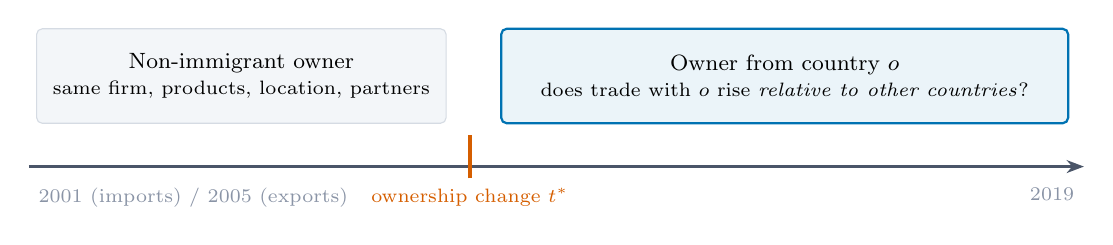
\begin{tikzpicture}
  \draw[line width=0.8pt,color=inksoft,-{Stealth[length=2.2mm]}] (0,0) -- (13.4,0);
  \node[bx,minimum width=5.2cm,minimum height=1.2cm] at (2.7,1.15)
     {Non-immigrant owner\\ \scriptsize same firm, products, location, partners};
  \node[bxkey,minimum width=7.2cm,minimum height=1.2cm] at (9.6,1.15)
     {Owner from country $o$\\ \scriptsize does trade with $o$ rise \emph{relative to other countries}?};
  \draw[owner,line width=1.4pt] (5.6,-0.15) -- (5.6,0.4);
  \node[font=\scriptsize,color=owner,below] at (5.6,-0.15) {ownership change $t^*$};
  \node[font=\scriptsize,color=mute,below right] at (0,-0.15) {2001 (imports) / 2005 (exports)};
  \node[font=\scriptsize,color=mute,below left] at (13.4,-0.15) {2019};
\end{tikzpicture}
\end{center}
\vspace{0.25cm}
\begin{columns}[T]
\begin{column}{0.31\textwidth}\begin{wordsbox}\textbf{Data}: customs records linked to owners, universe of traders\end{wordsbox}\end{column}
\begin{column}{0.31\textwidth}\begin{wordsbox}\textbf{Variation}: $\approx$1{,}000 switches from non-immigrant to immigrant owners\end{wordsbox}\end{column}
\begin{column}{0.31\textwidth}\begin{wordsbox}\textbf{Model}: maps 3 channels into distinct margin predictions\end{wordsbox}\end{column}
\end{columns}
\note[item]{Shapiro: convey why you have something to add: new linked data and a new source of variation.}
\end{frame}

%=====================================================================
\begin{frame}{Preview of findings}
\vspace{0.3cm}
\placeholder{After an owner from $o$ arrives, trade with $o$ rises by \_\_\% relative to other countries within \_\_ years; no pre-trend.}
\vspace{0.15cm}
\placeholder{The increase comes mainly from \_\_ (new country--product pairs / growth of existing flows), pointing to the \_\_ channel.}
\vspace{0.15cm}
\placeholder{The firm's trade becomes \_\_ concentrated; trade with other partners \_\_ (created / diverted).}
\note[item]{Shapiro: assume the audience is about to leave. Tangible but terse.}
\end{frame}

%=====================================================================
\divider{01}{Data}
%=====================================================================

\begin{frame}{Customs records linked to owners cover every Canadian goods trader}
\vspace{0.3cm}
\renewcommand{\arraystretch}{1.3}
\small
\begin{tabularx}{\textwidth}{@{}p{3.4cm}Xp{3.2cm}@{}}
\toprule
\textbf{Source} & \textbf{What it gives us} & \textbf{Years}\\
\midrule
TIC (imports) & firm $\times$ HS6 product $\times$ source country & 2001--2019\\
TEC (exports) & firm $\times$ HS8 product $\times$ destination (to HS6) & 2005--2019\\
CEEDD & firms, owners, employment & 2001--2019\\
IMDB & owner is an immigrant; country of origin & landings records\\
\bottomrule
\end{tabularx}
\vspace{0.4cm}
\begin{keybox}
\textbf{New here:} the owner's origin, linked to the full product-by-country trade portfolio, \emph{followed through a change of owner}.
\end{keybox}
\src{Merchandise trade only; values (no quantities). Main window 2005--2019 for both directions.}
\end{frame}

%=====================================================================
\begin{frame}{About 1,000 incumbent firms switch to immigrant owners}
\vspace{0.3cm}
\begin{columns}[T]
\begin{column}{0.5\textwidth}
\textbf{Event}: first year $t^*$ a firm passes to immigrant ownership; origin $o$ of the new owner.
\vspace{0.25cm}

\textbf{Not} conditioned on surviving or trading afterward.
\vspace{0.25cm}

\textbf{Excluded}: mergers, consolidations, identifier changes.
\end{column}
\begin{column}{0.44\textwidth}
\textbf{Comparison firms}
\vspace{0.1cm}
\begin{itemize}\setlength{\itemsep}{3pt}
\item never sold
\item sold to another non-immigrant\\ {\scriptsize\color{inksoft}same disruption of a sale}
\item sold to an immigrant from another origin\\ {\scriptsize\color{inksoft}same selection into immigrant ownership}
\end{itemize}
\end{column}
\end{columns}
\vspace{0.25cm}
\placeholder{Figure: number of switches by year and by origin region.}
\end{frame}

%=====================================================================
\divider{02}{Model}
%=====================================================================

\begin{frame}{The model in words: each trade relationship has to clear a bar}
\vspace{0.3cm}
\begin{wordsbox}[fontupper=\normalsize]
A firm already runs its business. For each \textbf{country} and \textbf{product}, it decides whether a trade relationship is worth having, and how much to trade through it.
\end{wordsbox}
\vspace{0.2cm}
\begin{columns}[T]
\begin{column}{0.31\textwidth}
\textbf{\ac{Fixed costs}}\\ {\small finding a partner, learning the rules, a first contract. Paid to \emph{have} a relationship.}
\end{column}
\begin{column}{0.31\textwidth}
\textbf{\ac{Variable cost}}\\ {\small contracting, monitoring, enforcement, shipping. Paid on every unit \emph{traded}.}
\end{column}
\begin{column}{0.31\textwidth}
\textbf{\hl{The owner from $o$}}\\ {\small knows part of what others must learn, \emph{for country $o$ only}.}
\end{column}
\end{columns}
\vspace{0.3cm}
\centering{\small Which cost the owner lowers determines \emph{how} the firm's trade with $o$ changes.}
\note[item]{Narrative first, then picture, then math (Cunningham ordering).}
\end{frame}

%=====================================================================
\begin{frame}{Fixed-cost cuts add relationships; variable-cost cuts grow them}
\vspace{0.1cm}
% Coordinate map (cm). Panel A origin (0,0); Panel B origin (7.6,0).
%  bars: width 0.6, x-left = 0.4 + 0.95*k (k=0..5); Panel B origin shifted to x=7.2
%  A heights 2.4,1.9,1.5,1.1,0.75,0.45 ; old cut y=1.3 ; new cut y=0.9
%  B old heights same (dashed) ; new heights x1.3 = 3.12,2.47,1.95,1.43,0.98,0.59 ; cut y=1.3
%  cut labels at x=6.05 (A) and x=13.65 (B), anchor west; A labels 0.4cm apart
%  panel titles at y=3.55 (A x=3.0, B x=10.6)
\begin{center}
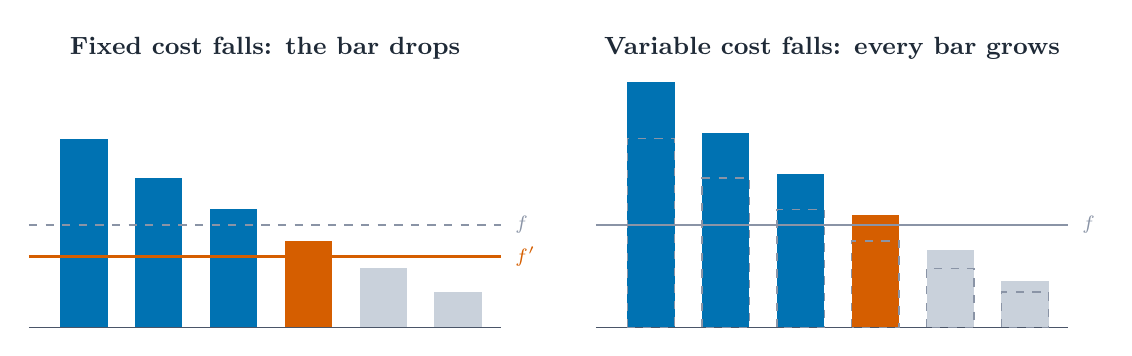
\begin{tikzpicture}
  % ---- Panel A
  \node[font=\small\bfseries,color=ink] at (3.0,3.55) {Fixed cost falls: the bar drops};
  \draw[color=inksoft,line width=0.6pt] (0,0) -- (6.0,0);
  \fill[barA] (0.40,0) rectangle (1.00,2.40);
  \fill[barA] (1.35,0) rectangle (1.95,1.90);
  \fill[barA] (2.30,0) rectangle (2.90,1.50);
  \fill[barN] (3.25,0) rectangle (3.85,1.10);
  \fill[barI] (4.20,0) rectangle (4.80,0.75);
  \fill[barI] (5.15,0) rectangle (5.75,0.45);
  \draw[cut,color=mute,dashed] (0,1.3) -- (6.0,1.3);
  \draw[cut,color=owner] (0,0.9) -- (6.0,0.9);
  \node[font=\scriptsize,color=mute,anchor=west] at (6.05,1.3) {$f$};
  \node[font=\scriptsize,color=owner,anchor=west] at (6.05,0.9) {$f'$};
  % ---- Panel B
  \node[font=\small\bfseries,color=ink] at (10.20,3.55) {Variable cost falls: every bar grows};
  \draw[color=inksoft,line width=0.6pt] (7.20,0) -- (13.20,0);
  \fill[barA] (7.60,0) rectangle (8.20,3.12);
  \fill[barA] (8.55,0) rectangle (9.15,2.47);
  \fill[barA] (9.50,0) rectangle (10.10,1.95);
  \fill[barN] (10.45,0) rectangle (11.05,1.43);
  \fill[barI] (11.40,0) rectangle (12.00,0.98);
  \fill[barI] (12.35,0) rectangle (12.95,0.59);
  \draw[barOld] (7.60,0) rectangle (8.20,2.40);
  \draw[barOld] (8.55,0) rectangle (9.15,1.90);
  \draw[barOld] (9.50,0) rectangle (10.10,1.50);
  \draw[barOld] (10.45,0) rectangle (11.05,1.10);
  \draw[barOld] (11.40,0) rectangle (12.00,0.75);
  \draw[barOld] (12.35,0) rectangle (12.95,0.45);
  \draw[cut,color=mute] (7.20,1.3) -- (13.20,1.3);
  \node[font=\scriptsize,color=mute,anchor=west] at (13.25,1.3) {$f$};
\end{tikzpicture}
\end{center}
\vspace{0.05cm}
{\footnotesize Bar = one product the firm could trade with $o$; height = variable profit.\\
\textcolor{accent}{$\blacksquare$}~active \quad \textcolor{owner}{$\blacksquare$}~newly active \quad \textcolor{inactive}{$\blacksquare$}~not worth it \quad dashed = before \quad line = the bar $f$}
\note[item]{Left: only new relationships appear; existing ones unchanged. Right: existing ones all grow by the same proportion, and a few marginal ones cross the bar.}
\end{frame}

%=====================================================================
\begin{frame}{Setup: a relationship pays variable profit minus fixed costs at two levels}
\vspace{0.15cm}
\begin{columns}[T]
\begin{column}{0.55\textwidth}
\begin{mathbox}
Relationship $(c,k,d)$: country $c$, product $k$, direction $d$
\[
\pi_{ickd} \;=\; \underbrace{\Phi_{ickd}\,\tau_{icd}^{-\varepsilon_d}}_{\text{variable profit}} \;-\; \underbrace{f_{ickd}}_{\text{product fixed cost}}
\]
plus a \textbf{country} fixed cost $F_{icd}$ if anything is traded with $c$.
\[
\Pi_i=\sum_{d}\sum_{c\in\mathcal C_{id}}\Big[\sum_{k\in\mathcal K_{icd}}\pi_{ickd}-F_{icd}\Big]
\]
\end{mathbox}
\end{column}
\begin{column}{0.39\textwidth}
\begin{wordsbox}
$\Phi$: firm scale, demand or supply in $c$, prices\\[0.2em]
$\tau$: variable cost of trading with $c$\\[0.2em]
$\varepsilon$: how much profit reacts to $\tau$\\[0.2em]
Trade value $X_{ickd}\propto\Phi\,\tau^{-\varepsilon}$
\end{wordsbox}
\vspace{0.15cm}
{\small\textbf{Rule}: trade product $k$ if $\Phi\tau^{-\varepsilon}\ge f$; trade with $c$ at all if the sum of those surpluses $\ge F$.}
\end{column}
\end{columns}
\note[item]{Relationships are separable in the baseline. The same reduced form covers exporters, importers for resale, and input importers (CES).}
\note[item]{This is the BRS two-tier fixed-cost structure at the level of one firm, with firm-specific costs.}
\end{frame}

%=====================================================================
\begin{frame}{The owner removes part of the \emph{information} cost, only for country $o$}
\vspace{0.15cm}
\begin{mathbox}
\vspace{-0.3cm}
\begin{align*}
\ln\tau_{icd} &= \ln\bar\tau_{cd} + (1-\hl{\lambda_\tau D_{ic}})\,\iota_c && \text{variable cost}\\
F_{icd} &= \bar F_{cd} + (1-\hl{\lambda_F D_{ic}})\,\psi_c && \text{country fixed cost}\\
f_{ickd} &= \bar f_{ckd} + (1-\hl{\lambda_f D_{ic}})\,\psi_{ck} && \text{product fixed cost}
\end{align*}
\end{mathbox}
\vspace{0.1cm}
\begin{columns}[T]
\begin{column}{0.47\textwidth}
\begin{wordsbox}
$D_{ic}=1$ if $c$ is the owner's origin.\\
$\bar\tau,\bar F,\bar f$: costs every Canadian firm faces.\\
$\iota,\psi$: the \emph{information} part. The owner removes a share $\lambda$ of it.
\end{wordsbox}
\end{column}
\begin{column}{0.47\textwidth}
\begin{wordsbox}
\textbf{Key assumption}: $\iota,\psi$ are larger where public information is scarce: differentiated goods, weak institutions, distant languages, thin Canada--$c$ trade.
\end{wordsbox}
\end{column}
\end{columns}
\note[item]{If the owner cut tau by a constant proportion everywhere, there would be no heterogeneity to test. The information component gives it.}
\end{frame}

%=====================================================================
\begin{frame}{The competing story: the owner shifts demand, not costs}
\vspace{0.4cm}
\begin{mathbox}
\[
\Phi_{ick,\mathrm{im}}=\bar\Phi_{ick,\mathrm{im}}\big(1+\hl{\eta}\,D_{ic}\,\one[k\ \text{consumer good}]\big)
\]
\end{mathbox}
\vspace{0.1cm}
\begin{wordsbox}
e.g.\ an owner serving co-ethnic customers imports more home-country consumer goods.
\end{wordsbox}
\vspace{0.25cm}
\begin{keybox}
\textbf{What makes it testable:} demand for home goods should \emph{not} raise exports to $o$ or imports of intermediate inputs from $o$.
\end{keybox}
\src{Weak point: co-ethnic demand for inputs, or an owner's trust in home suppliers, would look like a cost channel.}
\end{frame}

%=====================================================================
\begin{frame}{Margins separate fixed from variable costs; direction and goods separate costs from demand}
\vspace{0.15cm}
\footnotesize
\renewcommand{\arraystretch}{1.25}
\begin{tabularx}{\textwidth}{@{}>{\raggedright\arraybackslash}p{3.3cm}YYYY@{}}
\toprule
 & \textbf{Country fixed cost} & \textbf{Product fixed cost} & \textbf{Variable cost} & \textbf{Demand}\\
\midrule
Trade with $o$ vs.\ others & rises & rises & rises & consumer imports only\\
Existing $(o,k)$ flows & \hl{unchanged} & \hl{unchanged} & \ac{all grow by $\varepsilon\lambda_\tau\iota_o$} & consumer imports grow\\
New $(o,k)$ pairs & firms new to $o$, in bundles & one at a time & only near the bar & consumer goods\\
Exports \& input imports & rise & rise & rise & \hl{no change}\\
\bottomrule
\end{tabularx}
\note[item]{The margin separates fixed from variable costs; direction and goods type separate costs from demand.}
\note[item]{This table is the bridge to the empirics: every row is a regression.}
\end{frame}

%=====================================================================
\begin{frame}{Interacting sources do not break the within-firm comparison}
\vspace{0.2cm}
\begin{columns}[T]
\begin{column}{0.5\textwidth}
\begin{wordsbox}
A cheaper source lowers the firm's costs and raises its scale, which changes what it buys \emph{everywhere} (Antr\`as, Fort \& Tintelnot 2017).
\end{wordsbox}
\vspace{0.15cm}
\begin{mathbox}
\[
M_{ij}\;\propto\;T_j(\tau_{ij}w_j)^{-\theta}\;\Theta_i^{(\sigma-1-\theta)/\theta}
\]
\end{mathbox}
\end{column}
\begin{column}{0.44\textwidth}
\textbf{An owner who lowers $\tau_{io}$:}
\vspace{0.15cm}
\begin{itemize}\setlength{\itemsep}{5pt}
\item other countries all move by the \textbf{same proportion}, up if $(\sigma-1)/\theta>1$, down if $<1$
\item $o$ relative to any other country moves by exactly $\theta\lambda_\tau\iota_o$
\end{itemize}
\end{column}
\end{columns}
\vspace{0.3cm}
{\small Firm-by-year effects absorb the common part. \textbf{Creation vs.\ diversion} needs a comparison \emph{across} firms.}
\note[item]{$M_{ij}$: equation (12) in AFT; the separable baseline is their knife-edge case $(\sigma-1)/\theta=1$.}
\end{frame}

%=====================================================================
\begin{frame}{More trade with $o$ diversifies the firm only if $o$ starts out small}
\vspace{0.3cm}
\begin{columns}[T]
\begin{column}{0.47\textwidth}
\begin{mathbox}
Herfindahl across partners $H_i=\sum_c s_{ic}^2$
\[
\frac{\partial H_i}{\partial X_{io}}=\frac{2}{X_i}\big(\hl{s_{io}}-H_i\big)
\]
\end{mathbox}
\end{column}
\begin{column}{0.47\textwidth}
\begin{wordsbox}
Concentration falls when $o$'s share is below $H_i$.\\[0.3em]
For a firm dominated by the U.S., $H_i\approx$ U.S.\ share, so almost any non-U.S.\ origin diversifies it.
\end{wordsbox}
\end{column}
\end{columns}
\vspace{0.4cm}
\begin{keybox}
Firm-level and national diversification line up when the new trade is \emph{created}, not diverted from non-U.S.\ partners.
\end{keybox}
\end{frame}

%=====================================================================
\begin{frame}{Buyers may select on levels of opportunity, not on coming shocks}
\vspace{0.3cm}
\begin{wordsbox}[fontupper=\normalsize]
A buyer from $o$ values firm $i$ at $V_i+G_i(o)$. The gain $G_i(o)$ is larger for firms whose products $o$ supplies or buys.
\end{wordsbox}
\vspace{0.25cm}
\begin{columns}[T]
\begin{column}{0.47\textwidth}
\textbf{\ac{Fine for the design}}\\[0.15em]
{\small Selection on the \emph{level} of fit with $o$. Absorbed by firm $\times$ country $\times$ product effects. The estimand is the effect on acquired firms (ATT).}
\end{column}
\begin{column}{0.47\textwidth}
\textbf{\hl{Breaks the design}}\\[0.15em]
{\small Selection on a coming \emph{change}, e.g.\ a buyer who knows a contract with $o$ is in prospect.}
\end{column}
\end{columns}
\note[item]{This is the identifying assumption stated in economic terms (Shapiro: lay out economic assumptions that justify the econometric ones).}
\end{frame}

%=====================================================================
\divider{03}{Where the model comes from}
%=====================================================================

\begin{frame}{The model is assembled from standard, well-tested parts}
\vspace{-0.2cm}
% Coordinate map (cm):
%  left nodes center x=2.9, text width 5.4, min h=0.85; y = 4.32, 3.24, 2.16, 1.08, 0.0 (gap 1.08)
%  right node center (10.3,2.16) text width 4.6, min h=2.6
%  arrows: left.east -> right.west ; note at (2.9,4.95)
\begin{center}
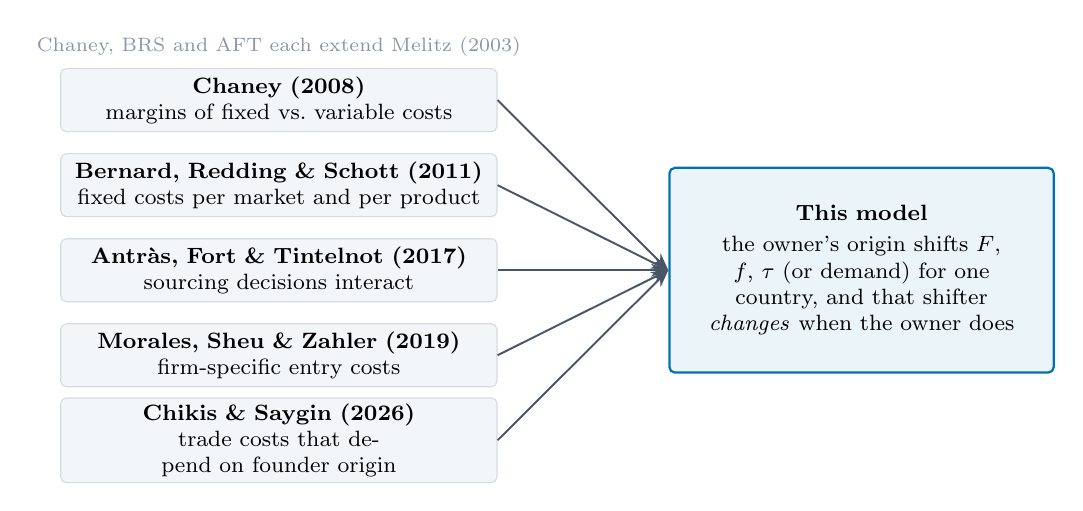
\begin{tikzpicture}
  \node[font=\scriptsize,color=mute] at (2.9,5.0) {Chaney, BRS and AFT each extend Melitz (2003)};
  \node[bx,text width=5.4cm,minimum height=0.8cm,inner sep=2pt] (c) at (2.9,4.32) {\textbf{Chaney (2008)}\\ margins of fixed vs.\ variable costs};
  \node[bx,text width=5.4cm,minimum height=0.8cm,inner sep=2pt] (b) at (2.9,3.24) {\textbf{Bernard, Redding \& Schott (2011)}\\ fixed costs per market and per product};
  \node[bx,text width=5.4cm,minimum height=0.8cm,inner sep=2pt] (a) at (2.9,2.16) {\textbf{Antr\`as, Fort \& Tintelnot (2017)}\\ sourcing decisions interact};
  \node[bx,text width=5.4cm,minimum height=0.8cm,inner sep=2pt] (m) at (2.9,1.08) {\textbf{Morales, Sheu \& Zahler (2019)}\\ firm-specific entry costs};
  \node[bx,text width=5.4cm,minimum height=0.8cm,inner sep=2pt] (s) at (2.9,0.0) {\textbf{Chikis \& Saygin (2026)}\\ trade costs that depend on founder origin};
  \node[bxkey,text width=4.6cm,minimum height=2.6cm] (me) at (10.3,2.16)
     {\textbf{This model}\\[0.2em] the owner's origin shifts $F$, $f$, $\tau$ (or demand) for one country, and that shifter \emph{changes} when the owner does};
  \foreach \n in {c,b,a,m,s} \draw[arr] (\n.east) -- (me.west);
\end{tikzpicture}
\end{center}
\note[item]{Honest positioning: nothing here is new machinery.}
\end{frame}

%=====================================================================
\begin{frame}{What is new is where the shifter enters, not the machinery}
\vspace{0.3cm}
\small
\begin{enumerate}\setlength{\itemsep}{4pt}
\item \textbf{A person-specific, partner-specific friction.} Costs differ by (owner origin, partner country), not only by country pair or by random draw.
\item \textbf{It moves within a firm.} An ownership change switches it on, which gives a testable event.
\item \textbf{Three channels in one setup} (fixed, variable, demand) with \emph{different} fingerprints, for imports \emph{and} exports, by product.
\item \textbf{Two results for the design}: interdependence is absorbed within firm; diversification has a simple condition, $s_{io}<H_i$.
\end{enumerate}
\vspace{0.05cm}
\begin{keybox}
Deliberately small: the aim is to tell channels apart with the data available, not to quantify welfare.
\end{keybox}
\end{frame}

%=====================================================================
\begin{frame}{No existing model pairs an owner-specific friction with a change in owner}
\vspace{-0.15cm}
\scriptsize
\renewcommand{\arraystretch}{1.08}
\begin{tabularx}{\textwidth}{@{}>{\raggedright\arraybackslash}p{2.0cm}>{\raggedright\arraybackslash}p{3.0cm}YYp{1.2cm}>{\raggedright\arraybackslash}p{1.7cm}@{}}
\toprule
 & \textbf{Firm-specific bilateral cost?} & \textbf{Where it comes from} & \textbf{Moves within the firm?} & \textbf{Direction} & \textbf{Many partners?}\\
\midrule
Chaney (2008) & no: $\tau_{ij},f_{ij}$ by country pair & n/a (productivity) & n/a & exports & yes\\
BRS (2011) & no: $F_{ij},f_{ij}$ by country pair & n/a (ability) & n/a & exports & yes, + products\\
AFT (2017) & in estimation only & random draws & no & imports & yes\\
MSZ (2019) & yes: sunk entry cost & its own past exports & yes, by own choices & exports & yes\\
CS (2026) & yes: search cost $\kappa_{on}$ & founder's birthplace & no (the founder) & imports & 1 country per input\\
\midrule
\textbf{This model} & \textbf{yes}: $F,f,\tau$ & \textbf{owner's origin} & \textbf{yes: new owner} & \textbf{both} & \textbf{yes, + products}\\
\bottomrule
\end{tabularx}
\end{frame}

%=====================================================================
\begin{frame}{Why the existing models could not answer this question as built}
\vspace{0.2cm}
\small
\begin{itemize}\setlength{\itemsep}{6pt}
\item \textbf{Chaney; BRS}: trade costs are the same for every firm in a country pair. Firm heterogeneity (productivity, ability) raises trade with \emph{all} partners, so it has no country of origin.
\item \textbf{AFT}: firm-by-country fixed costs appear only as random draws in estimation; nothing ties them to a person.
\item \textbf{MSZ}: closest in spirit, with firm-specific entry costs. But the knowledge comes from the firm's own past exports, which it chooses itself.
\item \textbf{CS}: costs tied to a person's origin, but the founder never changes and each input comes from one country, so there is no event and no partner count.
\end{itemize}
\vspace{0.15cm}
{\color{inksoft}\small Each could be extended to include an owner. The contribution is choosing where the shifter enters and deriving fingerprints that an ownership change can test.}
\end{frame}

%=====================================================================
\begin{frame}{Validation: the model reproduces its parents' results as special cases}
\footnotesize
\renewcommand{\arraystretch}{1.15}
\begin{tabularx}{\textwidth}{@{}>{\raggedright\arraybackslash}p{2.6cm}X>{\raggedright\arraybackslash}p{3.8cm}@{}}
\toprule
\textbf{Source result} & \textbf{What it says} & \textbf{Our counterpart}\\
\midrule
Chaney (2008) & fixed costs have zero intensive-margin elasticity; variable costs move both margins & fixed-cost channel leaves existing flows unchanged\\
BRS (2011) & fixed costs affect whether to supply, not sales once supplied & product and country cutoffs (Lemma 1)\\
AFT (2017) & at $(\sigma-1)/\theta=1$ adding one source does not affect adding others & our separable baseline\\
\bottomrule
\end{tabularx}
\vspace{0.15cm}
\textbf{Priors for $\lambda$}: shared language with a past destination cuts entry costs 29--36\% (MSZ); common language cuts fixed sourcing costs $\approx$13\% (AFT); birth-country search costs 33--78\% lower (CS).
\end{frame}

%=====================================================================
\begin{frame}{Where the model is weaker than its parents}
\vspace{0.4cm}
\begin{columns}[T]
\begin{column}{0.31\textwidth}
\begin{wordsbox}
\textbf{Static}\\[0.2em]
MSZ show that sunk costs and path dependence matter. Here, dynamics enter only through timing predictions.
\end{wordsbox}
\end{column}
\begin{column}{0.31\textwidth}
\begin{wordsbox}
\textbf{No prices}\\[0.2em]
CS see founders reach cheaper suppliers. With values only, search and variable-cost cuts look alike.
\end{wordsbox}
\end{column}
\begin{column}{0.31\textwidth}
\begin{wordsbox}
\textbf{Partial equilibrium}\\[0.2em]
No welfare or aggregate counterfactuals, unlike Chaney, AFT or CS.
\end{wordsbox}
\end{column}
\end{columns}
\vspace{0.4cm}
{\small MSZ's extended gravity also suggests an extension: the owner's knowledge may lower costs in countries \emph{similar} to $o$ (language, region).}
\end{frame}

%=====================================================================
\divider{04}{Empirical strategy}
%=====================================================================

\begin{frame}{Compare trade with $o$ to other countries, within firm and year}
\vspace{0.15cm}
\begin{mathbox}
\[
X_{ickt}=\exp\big(\hl{\beta}\,\Post_{it}\times\one[c=o_i]+\alpha_{it}+\gamma_{ckt}+\delta_{ick}\big)\,\epsilon_{ickt}
\qquad\text{(PPML, zeros kept)}
\]
\end{mathbox}
\vspace{0.1cm}
\footnotesize
\renewcommand{\arraystretch}{1.3}
\renewcommand{\arraystretch}{1.2}
\begin{tabularx}{\textwidth}{@{}p{4.6cm}X@{}}
\toprule
\textbf{Fixed effect} & \textbf{Absorbs}\\
\midrule
firm $\times$ year $\alpha_{it}$ & everything a sale changes for the whole firm: management, finance, scale\\
country $\times$ product $\times$ year $\gamma_{ckt}$ & tariffs, trade agreements, exchange rates, demand in $c$\\
firm $\times$ country $\times$ product $\delta_{ick}$ & persistent fit with $c$, including buyers' selection on levels\\
\bottomrule
\end{tabularx}
\vspace{0.1cm}
{\small\textbf{Identifying assumption}: absent the switch, trade with $o$ relative to other countries would have evolved as in comparison firms.}
\end{frame}

%=====================================================================
\begin{frame}{The event study and margin outcomes map onto the fingerprints}
\vspace{0.3cm}
\begin{columns}[T]
\begin{column}{0.47\textwidth}
\textbf{Event study}\\[0.15em]
{\small Stacked by cohort and origin, clean controls, event time $-4$ to $+6$. Robust to staggered timing.}
\vspace{0.3cm}

\textbf{Inference}\\[0.15em]
{\small Firm clusters plus randomization inference with placebo origins.}
\end{column}
\begin{column}{0.47\textwidth}
\textbf{Margins}
\begin{itemize}\setlength{\itemsep}{3pt}\small
\item country entry: trades with $o$ at all?
\item product breadth with $o$
\item new $(o,k)$ pairs
\item existing $(o,k)$ flows {\scriptsize(zeros kept; no survivor conditioning)}
\end{itemize}
\vspace{0.1cm}
\textbf{Across firms}: number of partners, HHI, non-U.S.\ share, third countries.
\end{column}
\end{columns}
\end{frame}

%=====================================================================
\begin{frame}{A skeptic: buyers pick firms about to trade with $o$ anyway}
\vspace{0.3cm}
\footnotesize
\renewcommand{\arraystretch}{1.35}
\begin{tabularx}{\textwidth}{@{}>{\raggedright\arraybackslash}p{4.3cm}X@{}}
\toprule
\textbf{Objection} & \textbf{Response}\\
\midrule
Buyer foresees growth with $o$ & event-study leads; drop switches with a pre-sale jump; compare with buyers from \emph{other} origins\\
Firms trading with $o$ attract buyers from $o$ & firm $\times$ country $\times$ product effects; results by pre-sale status\\
A sale reshuffles everything & firm $\times$ year effects; sales to non-immigrants as placebo\\
Early immigrants coded as non-immigrant & restrict by seller age; alternative ownership definitions\\
Fake origins would ``work'' too & placebo origins far from $o$ in language and region\\
\bottomrule
\end{tabularx}
\note[item]{Devil's advocate slide. Residual risk: selection on firm-and-o-specific shocks not visible in leads.}
\end{frame}

%=====================================================================
\divider{05}{Results}
%=====================================================================

\begin{frame}{[Result] Trade with the owner's origin rises after the switch}
\vspace{0.2cm}
\placeholder{Event-study figure, imports and exports side by side. Coefficients $\beta_e$ for $e\in[-4,6]$ with 95\% CIs and the number of treated firms at each horizon.}
\vspace{0.2cm}
{\small\textbf{How to read it}: flat leads support the design. A gradual rise points to fixed costs (search); a jump points to variable costs or demand.}
\end{frame}

\begin{frame}{[Result] The increase comes mainly through \_\_\_ margin}
\vspace{0.2cm}
\placeholder{Bar chart: effect on country entry, product breadth, new pairs, and existing flows, by direction.}
\vspace{0.2cm}
{\small\textbf{How to read it}: new pairs with flat existing flows point to fixed costs; proportional growth of existing flows points to variable costs.}
\end{frame}

\begin{frame}{[Result] Firms' trade becomes \_\_\_ concentrated}
\vspace{0.2cm}
\placeholder{Effects on number of partners, HHI, non-U.S.\ share, and trade with third countries (created vs.\ diverted).}
\vspace{0.2cm}
{\small\textbf{How to read it}: rising third-country trade means sources are complements (AFT); falling means diversion.}
\end{frame}

%=====================================================================
\begin{frame}[plain]
\vspace*{1.6cm}
\hspace*{0.6cm}{\color{accent}\rule{2cm}{2pt}}\par\vspace{0.4cm}
\hspace*{0.6cm}\begin{minipage}{0.85\textwidth}
{\Large\bfseries\raggedright If owners carry market knowledge, who owns Canada's firms shapes where Canada trades.\par}\par\vspace{0.6cm}
{\normalsize\color{inksoft}\raggedright\textbf{Bottom line:} an owner from $o$ is worth \_\_\% more trade with $o$, mostly through \_\_\_, and \_\_\_ the firm's concentration on the United States.}
\end{minipage}
\end{frame}

%=====================================================================
\appendix
\divider{A}{Appendix}
%=====================================================================

\begin{frame}{Chaney (2008): heterogeneous firms, fixed and variable export costs}
\vspace{0.15cm}
\begin{columns}[T]
\begin{column}{0.45\textwidth}
\textbf{Setup}\\[0.1em]
{\footnotesize Firms draw productivity $\varphi$ from a Pareto with shape $\gamma>\sigma-1$. Exporting from $i$ to $j$ costs iceberg $\tau_{ij}$ and fixed $f_{ij}$, the same for all firms in the pair. Only firms above a threshold $\bar\varphi_{ij}$ export.}
\vspace{0.2cm}

\textbf{Firm exports}: elasticity $\sigma-1$ with respect to $\tau_{ij}$.
\end{column}
\begin{column}{0.52\textwidth}
\begin{mathbox}
\footnotesize Margins of aggregate exports:
\[
\zeta\equiv-\tfrac{d\ln X_{ij}}{d\ln\tau_{ij}}=\underbrace{\sigma-1}_{\text{int.}}+\underbrace{\gamma-(\sigma-1)}_{\text{ext.}}=\gamma
\]
\[
\xi\equiv-\tfrac{d\ln X_{ij}}{d\ln f_{ij}}=\underbrace{0}_{\text{int.}}+\underbrace{\tfrac{\gamma}{\sigma-1}-1}_{\text{ext.}}
\]
\end{mathbox}
\end{column}
\end{columns}
\vspace{0.15cm}
{\small\textbf{Used here}: fixed costs move only the extensive margin. \textbf{Not here}: costs vary by country pair, not by owner.}
\src{Chaney, T. (2008), AER 98(4): Setup (eqs. 2--3), Propositions 1--2, Section III.}
\end{frame}

\begin{frame}{Bernard, Redding \& Schott (2011): fixed costs per market and per product}
\vspace{0.15cm}
\begin{columns}[T]
\begin{column}{0.45\textwidth}
{\footnotesize Firm ability $\varphi$ is common across products and countries. Product attributes $\lambda$ are idiosyncratic (common across countries, or country-specific). Serving market $j$ costs $F_{ij}$; each product there costs $f_{ij}$; trade costs are iceberg $\tau_{ij}$.}
\vspace{0.2cm}

{\footnotesize A product is supplied if $\lambda\ge\lambda^*_{ij}(\varphi)$; a market is served if the sum over profitable products covers $F_{ij}$.}
\end{column}
\begin{column}{0.52\textwidth}
\begin{mathbox}
\footnotesize Profits in market $j$ (eq.~9):
\begin{align*}
\pi_{ij}(\varphi)=&\int_{\lambda^*_{ij}(\varphi)}^{\infty}\Big(\tfrac{r_{ij}(\varphi,\lambda)}{\sigma}-w_if_{ij}\Big)z(\lambda)\,d\lambda\\
&-\,w_iF_{ij}
\end{align*}
\end{mathbox}
\end{column}
\end{columns}
\vspace{0.15cm}
{\small\textbf{Used here}: the two-tier fixed-cost structure; ``fixed costs affect whether to supply a market, not sales conditional on supplying.'' \textbf{Not here}: $F_{ij},f_{ij}$ are common to all firms from $i$ to $j$.}
\src{Bernard, Redding \& Schott (2011), QJE 126(3): Sections III.B--III.D, eqs. 6--10.}
\end{frame}

\begin{frame}{Antr\`as, Fort \& Tintelnot (2017): interdependent sourcing decisions}
\vspace{0.15cm}
\begin{columns}[T]
\begin{column}{0.53\textwidth}
{\footnotesize A firm pays $f_{ij}$ to be able to source from $j$. Its sourcing capability is $\Theta_i=\sum_{j\in\mathcal J_i}T_j(\tau_{ij}w_j)^{-\theta}$, and $j$'s share of input purchases is $T_j(\tau_{ij}w_j)^{-\theta}/\Theta_i$ (eqs.~7--8).}
\vspace{0.2cm}

{\footnotesize If $(\sigma-1)/\theta\ge1$, sources are complements: a lower $\tau_{ij}$ or $f_{ij}$ (weakly) raises purchases from \emph{all} countries (Prop.~3). In estimation, fixed costs vary by firm and country as lognormal draws whose scale depends on distance, language and corruption.}
\end{column}
\begin{column}{0.42\textwidth}
\begin{mathbox}
\small Profits (eq.~10):
\begin{align*}
\pi_i(\varphi)=&\,\varphi^{\sigma-1}(\gamma\Theta_i)^{\frac{\sigma-1}{\theta}}B_i\\
&-w_i\textstyle\sum_{j\in\mathcal J_i}f_{ij}
\end{align*}
\end{mathbox}
\end{column}
\end{columns}
\vspace{0.15cm}
{\small\textbf{Used here}: purchases scale with $\Theta_i$, so third-country effects are common across partners. \textbf{Not here}: an owner; exports.}
\src{Antr\`as, Fort \& Tintelnot (2017), AER 107(9); equation and proposition numbers from the resubmitted draft.}
\end{frame}

\begin{frame}{Morales, Sheu \& Zahler (2019): entry costs fall after similar markets}
\vspace{0.15cm}
\begin{columns}[T]
\begin{column}{0.53\textwidth}
{\footnotesize Chilean chemical exporters, 1995--2005. Dynamic choice of export destinations. Fixed costs $f_{ijt}$ depend on gravity. Sunk entry costs $s_{ijt}$ fall if the destination shares a border, continent, language or income level with a country the firm exported to \emph{last year} (``extended gravity'').}
\vspace{0.2cm}

{\footnotesize Estimated with moment inequalities, so the model is not solved and there are no counterfactuals.}
\end{column}
\begin{column}{0.42\textwidth}
\begin{mathbox}
\small Sunk entry cost (eqs.~11--13):
\[
s_{ijt}=s_j^o-e^o_{ijt}+\varepsilon^S_{ijt}
\]
\vspace{-0.4cm}

{\footnotesize $e^o_{ijt}$: extended-gravity reductions}
\end{mathbox}
\vspace{0.1cm}
{\footnotesize Jointly $-69$ to $-90\%$; geography $-25$ to $-38\%$; language $-29$ to $-36\%$.}
\end{column}
\end{columns}
\vspace{0.15cm}
{\small\textbf{Used here}: firm-specific knowledge lowers market-specific entry costs. \textbf{Not here}: knowledge from a person, imports, variable vs.\ fixed.}
\src{Morales, Sheu \& Zahler (2019), REStud 86(6): Section 3, abstract.}
\end{frame}

\begin{frame}{Chikis \& Saygin (2026): founder origin lowers supplier search costs}
\vspace{0.15cm}
\begin{columns}[T]
\begin{column}{0.53\textwidth}
{\footnotesize Agents choose wage work or entrepreneurship. An entrepreneur buys one input from one country $n$ and searches sequentially for suppliers. Each draw costs $P\kappa_{on}$ (founder origin $o$, source $n$). Lower $\kappa_{on}$: more selective search, cheaper inputs.}
\vspace{0.2cm}

{\footnotesize Sourcing odds identify relative search costs (Prop.~2), given equal domestic search costs. Birth-country search costs: 33--78\% below natives'.}
\end{column}
\begin{column}{0.42\textwidth}
\begin{mathbox}
\small Sourcing odds (eq.~15):
\[
\tfrac{\kappa_{on}/\kappa_{on'}}{\kappa_{o'n}/\kappa_{o'n'}}=\Big(\tfrac{\omega_{on}/\omega_{on'}}{\omega_{o'n}/\omega_{o'n'}}\Big)^{-\theta/\eta}
\]
\end{mathbox}
\vspace{0.1cm}
{\footnotesize Multi-input extension: one source per input (App.~B.6).}
\end{column}
\end{columns}
\vspace{0.15cm}
{\small\textbf{Used here}: person-origin-specific frictions. \textbf{Not here}: change of owner, exports, number of partners, fixed vs.\ variable costs.}
\src{Chikis \& Saygin (2026), job market paper: Sections 3.2--3.3, 4.}
\end{frame}

\begin{frame}{Threats to validity and responses}
\vspace{0.1cm}
\scriptsize
\renewcommand{\arraystretch}{1.25}
\begin{tabularx}{\textwidth}{@{}>{\raggedright\arraybackslash}p{3.4cm}>{\raggedright\arraybackslash}p{4.2cm}X@{}}
\toprule
\textbf{Threat} & \textbf{Why it matters} & \textbf{Response}\\
\midrule
Selection on future trade with $o$ & buyer foresees a contract & leads; drop pre-sale jumps; other-origin buyers; seller-initiated sales\\
Shocks to Canada--$o$ trade & trade agreements, tariffs & country $\times$ product $\times$ year effects\\
General effects of a sale & reorganization & firm $\times$ year effects; sales to non-immigrants\\
Network-driven matching & firms trading with $o$ attract buyers from $o$ & firm $\times$ country $\times$ product effects; split by pre-sale status\\
Owner mismeasurement & pre-coverage immigrants; mixed owners & seller age; ownership definitions\\
Zeros, large traders & logs drop zeros & PPML; participation; by size\\
Staggered timing & TWFE bias & stacked design; robust estimators\\
\bottomrule
\end{tabularx}
\end{frame}

\begin{frame}{Proofs in one line each}
\vspace{0.2cm}
\small
\begin{itemize}\setlength{\itemsep}{7pt}
\item \textbf{Margins.} Fixed-cost cuts leave $\Phi\tau^{-\varepsilon}$ unchanged, so existing flows are unchanged; only the cutoffs move. A variable-cost cut raises every $X_{iok}$ by $\varepsilon\lambda_\tau\iota_o$ in logs.
\item \textbf{Country fixed cost.} If $\Omega_{iod}\ge F_{iod}$ held already, nothing changes; otherwise entry activates every $k$ with $\Phi\tau^{-\varepsilon}\ge f$ at once.
\item \textbf{Diversification.} $H=\sum X_c^2/X^2\Rightarrow\partial H/\partial X_o=2(s_o-H)/X$.
\item \textbf{Interdependence.} $M_{ij}\propto T_j(\tau_{ij}w_j)^{-\theta}\Theta_i^{(\sigma-1-\theta)/\theta}$: a cut in $\tau_{io}$ scales all $j\neq o$ equally; $\ln M_{io}-\ln M_{ij}$ rises by $\theta\lambda_\tau\iota_o$.
\end{itemize}
\end{frame}

\end{document}
